\begin{figure}[]
\begin{tabular}{ccc}
\begin{subfigure}[b]{0.27\textwidth}
\begin{center}
{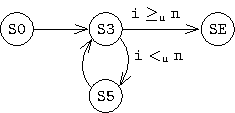
\includegraphics[scale=1]{chapters/figures/figMallocSpecCfg.pdf}}
\vspace{2pt}
\end{center}
\caption{\label{fig:llAllocSpecIRCFG}CFG of \SpecL{} Program}
\end{subfigure}%
&
\begin{subfigure}[b]{0.27\textwidth}
\begin{center}
{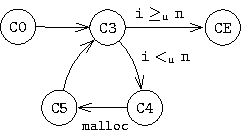
\includegraphics[scale=0.95]{chapters/figures/figMallocCCfg.pdf}}
\vspace{7pt}
\end{center}
\caption{\label{fig:llAllocCCFG}CFG of C Program}
\end{subfigure}%
&
\begin{subfigure}[b]{0.36\textwidth}
\begin{center}
{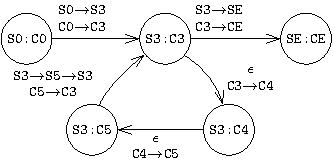
\includegraphics[scale=1]{chapters/figures/figMallocProductCfg.pdf}}
\end{center}
\caption{\label{fig:llAllocProductCFG}CFG of Product Program}
\end{subfigure}%
\\
\end{tabular}
\caption{\label{fig:mallocSpecCFGAndCCFG}CFG representation for Spec and C IRs shown in \cref{fig:llAllocSpecIR,fig:llAllocCIR}.\\ \Cref{fig:llAllocProductCFG} shows a product-CFG between the CFGs in \cref{fig:llAllocSpecIRCFG,fig:llAllocCCFG}.}
\end{figure}
